\section{Durchführung}
\label{sec:Durchführung}

\subsection{Aufbau}
Der Versuch besteht aus der Steuerelektronik, die das Eingangssignal in Spannung umwandeln kann. An die Steuerelektronik 
wird das Mikrofon, der PC der Lautsprecher und der Sinusgenerator angeschlossen.
\begin{figure}[H]
        \centering
        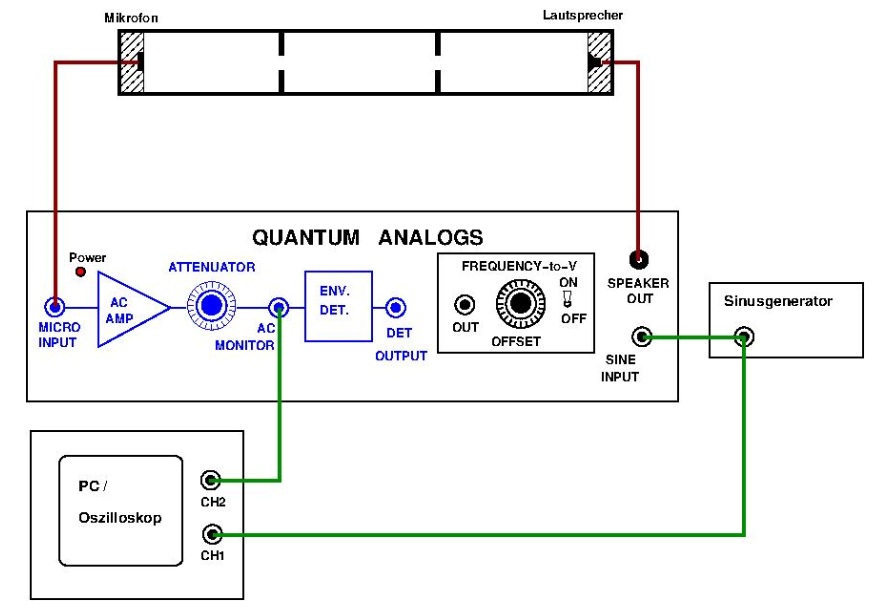
\includegraphics[width=0.8\textwidth]{content/pics/Schalt.png}
        \caption{Skizze des Schaltbildes~\cite{Durchfuhrung}.}
\end{figure}
Des Weiteren liegen verschieden große Zylinder vor. 
Mithilfe des Kugelresonators kann das Wasserstoffatom dargestellt werden, der Kugelresonator besteht hierbei aus zwei Halbkugeln 
wobei eine als Mikrofon und eine als Lautsprecher fungiert. 
Außerdem gibt es $3$ Zwischenringe mit den Dicken $\qty{3}{\milli\meter}$, $\qty{6}{\milli\meter}$ und $\qty{9}{\milli\meter}$ zur Aufbrechung der Kugelsymmetrie.
\begin{figure}[H]
        \centering
        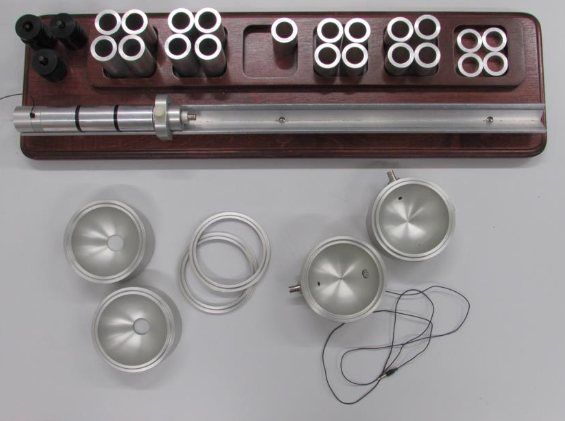
\includegraphics[width=0.8\textwidth]{content/pics/Auf.png}
        \caption{Baukasten des Versuchaufbaus~\cite{Durchfuhrung}.}
\end{figure}

\subsection{Vorbereitende Experimente}
Hierbei wird in die Schiene zwischen Lautsprecher und Mikrofon anfangs ein \qty{75}{mm} Zylinder gelegt. 
Das Frequenzspektrum auf dem PC wird von \qty{100}{Hz} bis \qty{12}{kHz} gestellt.
Die Messung wird solange mit je einem weiteren \qty{75}{mm} Zylinder wiederholt, bis die Schiene voll ist. 
Für Zylinder der Länge \qty{50}{mm} wird diese Messreihe wiederholt. 

\subsection{Wasserstoffatom}
Hierbei werden die zwei Kugelhälften als Kugelresonator verwendet. Anfangs wird bei einem Winkel $\alpha = \qty{180}{\degree}$ 
ein Frequenzspektrum von \qty{100}{Hz} bis \qty{12}{kHz} aufgenommen zur Bestimmung der Resonanzfrequenzen.
Im Folgenden wird für mindestens 4 dieser Resonanzfrequenzen ein hochauflösendes Frequenzspektrum aufgenommen. 
Es wird hierbei jeweils der Winkel in \qty{5}{\degree} Schritten von \qty{0}{\degree} auf \qty{180}{\degree} variiert.
Im Anschluss wird ein \qty{3}{mm} Zwischenring zwischen die obere und untere Kugelhälfte gesetzt. Der Winkel wird auf \qty{180}{\degree} 
gestellt und es wird ein hochauflösendes Frequenzspektrum zwischen \qty{1.8}{kHz} und \qty{2.6}{kHz} aufgenommen. Diese Messung wird 
wiederholt für einen \qty{6}{mm} Messring und der Kombination aus dem \qty{3}{mm} und \qty{6}{mm} Messring.
Des Weiteren wird für den \qty{9}{mm} Messring die Winkelabhängigkeit der Amplitude vermessen bei der Resonanzfrequenz von \qty{2.3}{kHz}.


\clearpage